\documentclass[a4paper,10pt]{article}
\usepackage{graphicx}
\usepackage[english]{babel}
\usepackage[latin1]{inputenc}
\usepackage{hyperref}
\usepackage{amsmath}
\usepackage{float}
\begin{document}
   \title{Analysis of D-Ary Heaps through Dijkstra's Shortest Path Algorithm}

   \author{Joshua Tensuan \\ e-mail: joshua.tensuan99@gmail.com}
          
   \date{}

   \maketitle
   
   \tableofcontents
 
  \newpage

\section*{Foreword}
In our code, the daryheap.cpp and daryheap.h file is where the d-ary heap class is implemented. The graph.h file is where Dijkstra's shortest path algorithm is implemented. We use and execute the class in the main.cpp file. The soc-pokec-relationships.txt file contains the data used for generating the graph. Details of the dataset can be found in the readme.txt file. \smallbreak
The following report will be organized and subdivided in four sections: \textbf{I}ntroduction, 
\textbf{M}ethods, \textbf{R}esults \textbf{A}nd \textbf{D}iscussion. In the introduction, we discuss basic definitions for d-ary heaps and Dijkstra's algorithm and applications for them, as well as addressing our basic goal. In our methods section, we detail more specific implementation of our d-ary heap class into Dijkstra's algorithm and our methods for timing and gathering runtime results. In our results section, we show a table of various d values and the corresponding runtime for Dijkstra's algorithm. Finally, in our discussion section, we talk about the effects of our results and future directions this project can take from here.

\section{Introduction} 
A heap is a special tree-based structure that follows 2 conditions: (1) the tree is complete and (2) the key of a parent node is less than both of the keys of the child nodes (in a min heap). Typically, heaps are implemented as binary in which parents have a max of 2 children. However, heaps can be modified so that parent nodes can have a different number of child nodes. These heaps are generally termed d-ary heaps where d is the max amount of child nodes per parent node. \smallbreak
There are many innovative use cases where one can use a heap. Priority queues, for example, often use heaps. Priority queues can then be used with many applications such as Dijkstra's shortest path algorithm, Prim's algorithm, Huffman encoding, and load balancing. In this specific project, we take a look at the implementation of d-ary heaps with Dijkstra's shortest path algorithm. With Dijkstra's algorithm, we seek an optimal d number such that the algorithm runs in the fastest runtime. \smallbreak
In general, shortest path algorithms are algorithms that find the shortest path between two points on a given graph. There are many applications for shortest path algorithms such as map route finding, computer networking, and spreading of an infectious disease. One popular algorithm for finding the shortest path for a single source is Bellman-Ford's algorithm. The general pseudocode for Bellman-Ford's algorithm is as follows \cite{bellman}:
\begin{verbatim}
 function BellmanFord(list vertices, list edges, vertex source)
   ::distance[],predecessor[]
   
   // This implementation takes in a graph, represented as
   // lists of vertices and edges, and fills two arrays
   // (distance and predecessor) about the shortest path
   // from the source to each vertex
   
   // Step 1: initialize graph
   for each vertex v in vertices:
       distance[v] := inf    // Initialize the distance to all vertices to infinity
       predecessor[v] := null         // And having a null predecessor
   
   distance[source] := 0  // The distance from the source to itself is, of course, zero
   
   // Step 2: relax edges repeatedly
   for i from 1 to size(vertices)-1:
       for each edge (u, v) with weight w in edges:
           if distance[u] + w < distance[v]:
               distance[v] := distance[u] + w
               predecessor[v] := u
   
   // Step 3: check for negative-weight cycles
   for each edge (u, v) with weight w in edges:
       if distance[u] + w < distance[v]:
           error "Graph contains a negative-weight cycle"
   
   return distance[], predecessor[]
\end{verbatim}

This algorithm has runs in $\mathcal{O}(\lvert V \rvert * \lvert E\rvert)$ in which V is the number of nodes and E is the number of edges. Dijkstra's algorithm serves as a faster alternative and instead runs in $\mathcal{O}(\lvert E\rvert \log{}\lvert V \rvert)$. The general pseudocode for Dijkstra's algorithm with a priority queue is as follows \cite{dijkstra}:
\begin{verbatim}
   function Dijkstra(Graph, source):
   dist[source] ← 0                           // Initialization
 
   create vertex priority queue Q
 
   for each vertex v in Graph:           
       if v ≠ source
           dist[v] ← INFINITY                 // Unknown distance from source to v
       prev[v] ← UNDEFINED                    // Predecessor of v
  
       Q.add_with_priority(v, dist[v])
  
  
   while Q is not empty:                      // The main loop
       u ← Q.extract_min()                    // Remove and return best vertex
       for each neighbor v of u:              // only v that are still in Q
           alt ← dist[u] + length(u, v) 
           if alt < dist[v]
               dist[v] ← alt
               prev[v] ← u
               Q.decrease_priority(v, alt)
  
   return dist, prev
\end{verbatim}

We implement Dijkstra's algorithm using a d-ary heap for the priority queue in the language C++. Using this, we test Dijkstra's algorithm runtime on a large network dataset (will expand in methods) with various d values to find the optimal d to maximize efficiency.
% Dijkstra's shortest path algorithm is an algorithm that finds the shortest path between two points on a given graph. 
 
 
\section{Methods}
The methods section is divided into several subsections. In subsection 2.1, we discuss the implementation of the d-ary heap in C++. In subsection 2.2, we discuss the implementation of Dijkstra's shortest path algorithm with the d-ary heap mentioned in subsection 2.1, as well as the implementation of a large network dataset. In subsection 2.3, we discuss our way of gathering and analyzing runtime data.
\subsection{D-Ary Heap Implementation}
The d-ary Heap was implemented in its own separate file. The heap was implemented using a vector of integer pairs, which allows us to easily change the size of the heap. In this integer pair, the first value represents the node the connection is going to, and the second value represents the weight of that connection. The d-ary heap constructor takes in a parameter d which sets the number of branches that can come out of a single parent node. A sift up method was implemented that takes in an index of where to sift up from. A sift down method was also implemented that takes in an index of where to sift down from and an index of where to bound the sift down. The d-ary heap is sorted by the second element of the integer pair where the parent's key will be smaller than a child's key (standard min heap). For Dijkstra's algorithm, this lets us sort to find the minimum distance. 
\subsection{Dijkstra's Shortest Path Algorithm Implementation}
Dijkstra's algorithm takes a graph and a node, and gives the shortest path between the given node and every other node in the graph. In this project, we store the graph in an adjacency list representation which is more efficient than an adjacency matrix as it decreases the memory the algorithm takes up as there are often many 0s (that are useless) in any given adjacency matrix for a graph. Our Dijkstra's algorithm was implemented in a different file. The shortest path method takes in a parameter for the node to start from and a d to construct the d-ary heap. We then take the shortest path from the source node to every node in the graph and place it in a text file named outfile.txt where a distance of 1 means there is only one connection between the nodes (2 means 2 connections etc.). The value of 1061109567 was used as a large (approximation for infinity) distance in our algorithm. When this value appears in our outfile.txt, it means there is no possible path between the source and that node. \smallbreak
After implementing Dijkstra's algorithm and testing it with a small graph, we then moved to testing it on larger datasets. For this project, we used a graph of the Pokec social network gathered from the Stanford Network Analysis Project's large network dataset \cite{snap}. The Pokec social network is similar to Facebook but smaller in size but has still connected over 1.6 million users for more than 10 years \cite{takoc}. It  offers chat, e-mail,  picture  and  video  sharing  services. Pokec is  the  most popular social network in Slovakia and is very popular in the Czech Republic as well. The graph we use represents every user and the connection represents a friend connection (these friend connections are directed and unweighted). In total, there are 1632803 nodes and 30622564 edges in our graph. Every weight was initialized as 1 as the graph is an unweighted graph. 

\subsection{Gathering Data}
    To time our data, we used the default chrono package from C++. For every d, we averaged out the runtimes for 5 runs of the shortest path algorithm. In this project, we analyzed values of d from 2 to 16. We also tested values of d far outside of the bounds, (30, 50, 100 etc.), but we noticed that these runtimes were significantly slower than values of d between 2 and 16 so they are not included in our results section. During the timing process, we made sure to only have the terminal that was running the code open to limit the effect of outside processes on the CPU load and performance. We then recorded the runtimes in seconds into an excel sheet and made scatterplot with it. With this scatterplot, we can then approximately deduce the optimal d-value. \smallbreak
    The implementation of Bellman-Ford's algorithm was attempted to cross-reference the shortest path output of Dijkstra's algorithm, but the algorithm itself took too long with a runtime of $\mathcal{O}(\lvert V \rvert * \lvert E\rvert)$. To provide some verification that Dijkstra's algorithm was right, we tested the algorithm on smaller networks and found that it worked correctly and as intended. Further, the Stanford Network Analysis Project that provided us with the dataset gave the longest shortest path as 11. We then looked through the output file of Dijkstra's shortest path algorithm and ensured that 11 was the longest shortest path possible (all other paths were less than or equal to a distance of 11 or equal to infinity (1061109567)).

\bigskip
\bigskip
\bigskip

\begin{center}
    \large
    Continue to next page for rest of the paper. Rest of page left blank to make formatting easier and nicer.
\end{center}
\newpage
\section{Results}
We got the following runtimes for Dijkstra's algorithm for various values of d:

{\centering
\begin{table}[H]
\begin{tabular}{|c|c|}
\hline
\textit{d} & \textit{time (s)} \\ \hline
2          & 10.836            \\ \hline
3          & 10.084            \\ \hline
4          & 9.668             \\ \hline
5          & 9.629             \\ \hline
6          & 9.517             \\ \hline
7          & 9.178             \\ \hline
8          & 8.893             \\ \hline
9          & 9.154             \\ \hline
10         & 9.281             \\ \hline
11         & 9.371             \\ \hline
12         & 9.544             \\ \hline
13         & 9.691             \\ \hline
14         & 9.546             \\ \hline
15         & 9.383             \\ \hline
16         & 9.5               \\ \hline
\end{tabular}
\end{table}
}
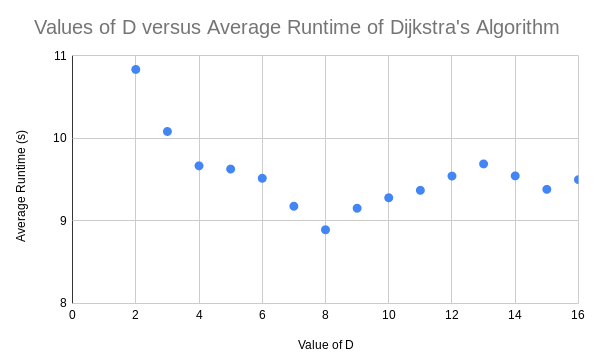
\includegraphics{graph.png}

\newpage

\section{Discussion}
Based off our results, we see a dip in the runtime with a d value of 8. With this, we can conclude that the optimal value of d for Dijkstra's shortest path algorithm with a heap is 8. \smallbreak
However, there are many possible sources of error that could have occurred with this project. For example, other processes could have been running at the same time which would interfere with the runtime. This could be resolved by redoing the experiment in a more isolated environment with an empty computer. Further, more trials could have been run to reduce the effects the standard deviation between runtimes for each value of d.  \smallbreak
There are many exciting directions this project can take from here. For example, with an optimal d-ary heap, we can then apply Dijkstra's shortest path algorithm to solve many real problems as discussed in section 1. We can also apply the same process to find the optimal value of d for other d-ary heap ans priority queue applications as discussed in section 1 as well. Currently, we have little insight into why the ideal value for the d-ary heap in Dijkstra's shortest path algorithm is 8. Hopefully with future research, we can mathematically deduce why 8 is the ideal value.

\begin{thebibliography}{}
    % references could have been nicer but good enough
  \bibitem{bellman} 
    \url{https://en.wikipedia.org/wiki/Bellman-Ford_algorithm};

   \bibitem{dijkstra} 
    \url{https://en.wikipedia.org/wiki/Dijkstra's_algorithm};
   \bibitem{snap} Jure Leskovec and Andrej Krevl,
    SNAP Datasets: Stanford Large Data Network Collection,
    \url{http://snap.stanford.edu/data}
   \bibitem{takoc} Takoc, L. \& Zabovsky, M. 2012,
       Data Analysis in Public Social Networks,
       \url{https://snap.stanford.edu/data/soc-pokec.pdf}
\end{thebibliography}

\end{document}

